\documentclass[tesis.tex]{subfiles}
\begin{document}
    
\section{Discussion}

When the mouth of an estuary is closed, it can become vertically stratified due to the freshwater input and the occasional wave overtopping of saline water. In such circumstances, it becomes difficult to energize the water column. However, external factors such as wind stress on the surface, discharge and wave overtopping can cause vertical transport in the water column (Roberts et al., 2021). In the case of Pescadero, vertical transport could not be driven by density exchange, as the estuary would always be saltier than the input water from the creeks, resulting in a consistently stratified water column. Nevertheless, there exists a light density/salinity gradient in Pescadero due to the freshwater input from upstream and saltwater overtopping the bar at the other end.\\

\subsection{Estuarine structure and morphology}

During the winter of 2012 Pescadero estuary received less fresh water inflow compared to other months throughout the year, leading the inlet to disconnect from the ocean. Pescadero during its closed state function as a stratified coastal lagoon with river runoff forming a surface layer of fresh water and occasionally having tidal inflows of saline water. The orientation of the bay and the shallowness result in the exposure of all the water columns to the wind stress events. In this regard, Pescadero shares many physical traits with other bar-built estuaries where the local wind forcing is the dominant driver.\\

Apart from the stratification, there is an along-estuary density gradient between the outlet of the creek and the mouth, due to the constant discharge of freshwater. Near the mouth, the upper layer is thinner than in the creek's outlet, probably because the salinity is higher in the mouth due to the waves that are overtopping the sandbar along with upstream continuous freshwater input.\\

The present study analysis reported that the major driver of mixing is wind stress and the major driver of water level variability is freshwater inflow, even in periods when is very low. In the next sections, we are going to discuss the role of other factors that affect Pescadero and its importance in stratification and water level.\\

\subsection{Analysis methods}

Wind and estuarine velocities were axis-rotated in the direction of maximum variance of water currents (See Fig. \ref{fig:rotacion}, Section \ref{Estuary_currents}), but there was also the option of doing it in the direction of wind velocity. This puts the main focus on the estuary currents instead of the wind velocity, but in this particular case, both, wind and water velocities, have a similar principal direction, so it wouldn't be a big difference between each option.\\

We adjusted the first cell of the ADCP data by visual inspection, using the blank space given by the ADCP, which was 0.71 m, and overlapping it with the CTD data on the same location DC. This comparison gave us the value of 0.91 m for the first cell location, which is merely an estimation, so it could have been a different value, bigger or smaller depending on how we had placed the overlapping. This does not affect velocity values, but we have to consider it for the positions of the layers or the profiles, but it does not make an important change in the analysis.\\

The closed state definition was set in a range of depth's change in time values with a 10-hour frame. The frame was selected by trial and error based on the timescale we were working on and it could change depending on the period in which the data was collected and the data collection frequency. Also, we have to consider that the opening and closures do not happen in an instant, but in a process that could last from minutes to hours, so it could be considered any instant during that process. In this case, the registered openings lasted 4, 21 and 28 hours each.\\ 

In this study, we did not consider temperature and evaporation factors. We considered that the effect of temperature was not important due to the haline stratification that dominated the estuary, but it could be studied in greater depth in future analyzes in Pescadero. Also, we didn't consider evaporation as a factor for depth changes because we are studying an estuary with a small area, and as it was winter time the air temperature was not too high to cause major impacts.\\

To calculate wind stress we used a drag coefficient defined by \cite{large1981open}, but according to \cite{paugam2021wind} the drag coefficient $C_D$ can be difficult to estimate in shallow water, so we have to consider the obtained $C_D$ as an approximation in the wind stress and everything calculated with that coefficient. In future studies, there could be used other drag coefficients to observe if there is a big difference in the wind stress and other indices obtained with $C_D$.\\

The Wedderburn number was obtained with the equation for a rectangular basin defined by \cite{Monismith1985}, so it is showing us an approximated value. Despite this, it is still a good indicator to estimate the behavior of the stratification to wind stress. We could try in future research more adapted Wedderburn numbers to the Pescadero basin and compare the results with those obtained in this study.\\

The frequency spectral analysis only shows a general view of the most important frequencies in the dataset but does not show the specific time when this happens. This makes it a special tool to detect frequency peaks and contrasting different datasets.\\

\subsection{Wind stress mixing}

% When the mouth of an estuary is closed, it results in a vertically stratified water column, which is fed by freshwater input and sporadic wave overtopping saline water. In such circumstances, it becomes difficult to energize the water column. However, external factors such as wind stress on the surface, discharge and wave overtopping can cause vertical transport in the water column (Roberts et al., 2021). In the case of Pescadero estuary, vertical transport could not be achieved through density-driven exchange as the estuary would always remain stratified due to the saltwater being denser than the freshwater input. Nevertheless, there exists a slight density/salinity gradient in Pescadero due to the freshwater input upstream and saltwater overtopping the bar at the other end (Shintani et al., 2010).

% The stratification of an estuary plays a significant role in the exchange processes between the estuary and adjacent water bodies. For example, in Lake Tahoe, stratification prevents the oxygenated water from mixing with the hypolimnion water, leading to the depletion of dissolved oxygen in the hypolimnion, which can affect the aquatic life (Schladow et al., 2018). Similarly, in San Francisco Bay, stratification results in the accumulation of contaminants in the bottom water leading to adverse impacts on the benthic community (Cloern et al., 2014).

% In Pescadero, the setup and relaxation of spring upwelling have been studied by Roberts et al. (2021). The authors found that spring upwelling can induce mixing in the water column, which can reduce the stratification of the estuary. However, the study also showed that the relaxation of upwelling can lead to the re-stratification of the water column. Shintani et al. (2010) proposed the use of the generalized Wedderburn number as a parameter to quantify upwelling in stratified lakes. The Wedderburn number is a measure of the buoyancy flux and can be used to evaluate the efficiency of vertical mixing in the water column. The study showed that the Wedderburn number can be a useful tool to predict the onset of upwelling in stratified lakes.

% In conclusion, the stratification of water bodies plays a crucial role in the exchange processes between adjacent water bodies. The vertical transport in the water column can be achieved through external factors such as wind stress on the surface, discharge and wave overtopping. The use of the generalized Wedderburn number can be a useful tool to predict the onset of upwelling in stratified lakes. Future research should focus on improving our understanding of the dynamics of stratified water bodies and its implications on the aquatic life.

% References:

% Cloern, J. E., Thompson, J. K., Hieb, K. A., Lopez, C. B., & Cole, B. E. (2014). Delta smelt: Life history and decline of a once-abundant species in the San Francisco Estuary. San Francisco Estuary and Watershed Science, 12(2).
% Roberts, D. C., Egan, G. C., Forrest, A. L., Largier, J. L., Bombardelli, F. A., Laval, B. E., Monismith, S. G., and Schladow, G. (2021). The setup and relaxation of spring upwelling in a deep, rotationally influenced lake. Limnology and Oceanography, 66(4):1168–1189.
% Schladow, S. G., Reuter, J. E., Coats, R., Heyvaert, A. C., & Det

Strong wind events were an important part of estuarine dynamics in Pescadero, inducing changes in circulation and stratification. Between November and January, sporadic strong wind events were recorded, with 3 to 4 events per month. However, during the study period, an increase in the occurrence of these wind events was observed, reaching between 7 and 8 events per month \ref{fig:velwind2}. \\

\begin{figure}[h!]
    \centering
    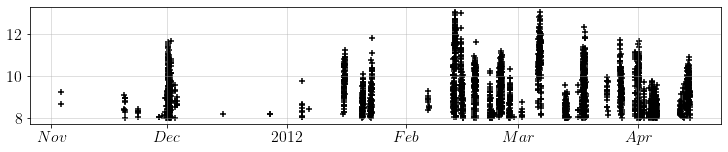
\includegraphics[width=\textwidth]{Imagenes/viento_fuerte.png}
    \caption{Occurrence of strong wind events in Pescadero estuary.}
    \label{fig:velwind2}
\end{figure}

Sporadic abrupt changes in density along the water column in different locations were apparent during the periods of the closed state. These sudden changes indicate that they were not caused by gradual processes, but rather resulted from sporadic events that are attributed to the effects of wind stress present at the same time as the density changes. After these events, density did not return to its original values from before the event so mixing was present in the three studied locations.\\

Fig. \ref{fig:perfiles2} is showing density profiles in the studied locations before (in red) and after (in cyan) a big wind event, showing a difference in the density values, especially in the bottom where there is a decrease in density. Buoyancy frequency showed a decrease after the wind event meaning a change in stratification, same as the potential energy anomaly in Fig. \ref{fig:phi}. Also in Fig. \ref{fig:diff} $\Delta \rho/\Delta z$ is showing a decrease in stratification between before and after big wind events, only observing this abrupt change twice, with one time during each closed state period.\\

We chose to obtain a range of values for the Wedderburn number as we did not know the exact placement of the pycnocline. Due to the constant freshwater inflow, the stratification of the estuary is changing over time, which means the surface layer is also changing its thickness. The range limits of W were obtained as a function that depends directly on the water level. We assumed the density interface theoretically reaches the upwind surface at W = 1, so if the full range of W goes lower than that value we will consider it a full upwelling. During a full upwelling, if we consider a linear tilt, the lower limit reaches the surface, different from partial upwelling, where just the upper limit reaches the surface. The main difference between both events of upwelling is that the full one is changing the density structure and the other one is not. We can observe this in Fig. \ref{fig:phi} where the potential energy anomaly after the partial upwelling events is not changing. During the upwelling events, there is the presence of baroclinic pressure gradients which increase with a lower W, so during the partial upwelling events, the gradients are not enough to mix the water column and change the stratification structure.\\

On the other hand, we observed surface fluctuations during the wind events, which are noticeable in the wavelet analysis in Fig. \ref{fig:surf2}. Also, there is a small relation between wind and depth density frequencies (Fig. \ref{fig:freq}) around a period of 200 min.\\

\subsection{Wind-driven circulation}

During and after wind events there were observed circulation processes that are indicating how the layers of the estuary behave. We already noticed that the main driver of changes in velocity in the estuary is wind stress. In Fig. \ref{fig:velwind} we observed with more detail the circulation occurring around the first wind event of the second period. We observed that the estuary had some circulation occurring before the event, when there is no wind stress, due to the constant freshwater inflow that is present in Pescadero. This velocity is positive (streamflow direction) and is at the superior layer detected by the ADCP. Also, before the wind event, with $\tau_w =0$, there was a negative velocity at the top of the range occurring at the same time as a detected wave overtopping event, meaning that the waves were creating a small circulation in the surface of the estuary that was overlapping the discharge velocity.\\

\begin{figure}[h!]
    \centering
    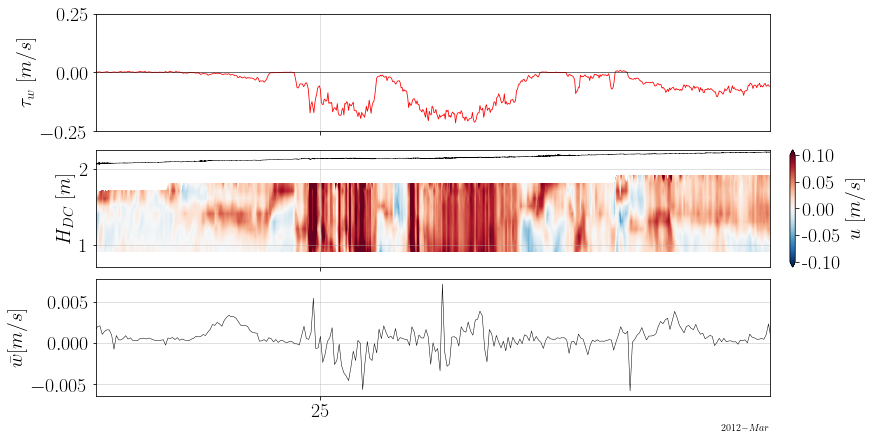
\includegraphics[width=\textwidth]{Imagenes/vel_wind.png}
    \caption{Time-series of wind stress ($\tau_w$), along-estuary velocity in the water column, along-estuary velocity in the upper and lower layers of the ADCP range, and depth wavelet frequency analysis at DC and tidal height in San Francisco (gray). }
    \label{fig:velwind}
\end{figure}

During the wind event, we observed an increase in velocity in the positive direction, while the wind stress is negative. The literature says that a stratified waterbody that is subjected to surface stress has its surface layer circulating with the same direction of the wind with a set-up of the free surface at the leeward zone, depressing the pycnocline and resulting in set-down at the wind leeward shore and circulation of the lower layer in the opposite direction of the wind \citep{Katopodes2018}. Despite the last statement we observed in Fig. \ref{fig:velwind} the velocity during a wind event is in the opposite direction of the wind. This is due to the range of available data from the ADCP, which starts measuring at 0.91 m and doesn't work near the surface, not showing the surface layer circulation and skipping the part where the velocity is in the same direction as the wind. Also, when the wind blows, the upper layer moves towards the surface and upstream moving away from the detected range (Fig. \ref{fig:adcp}) making the upper layer thinner at the DC location.\\

\begin{figure}[h!]
    \centering
    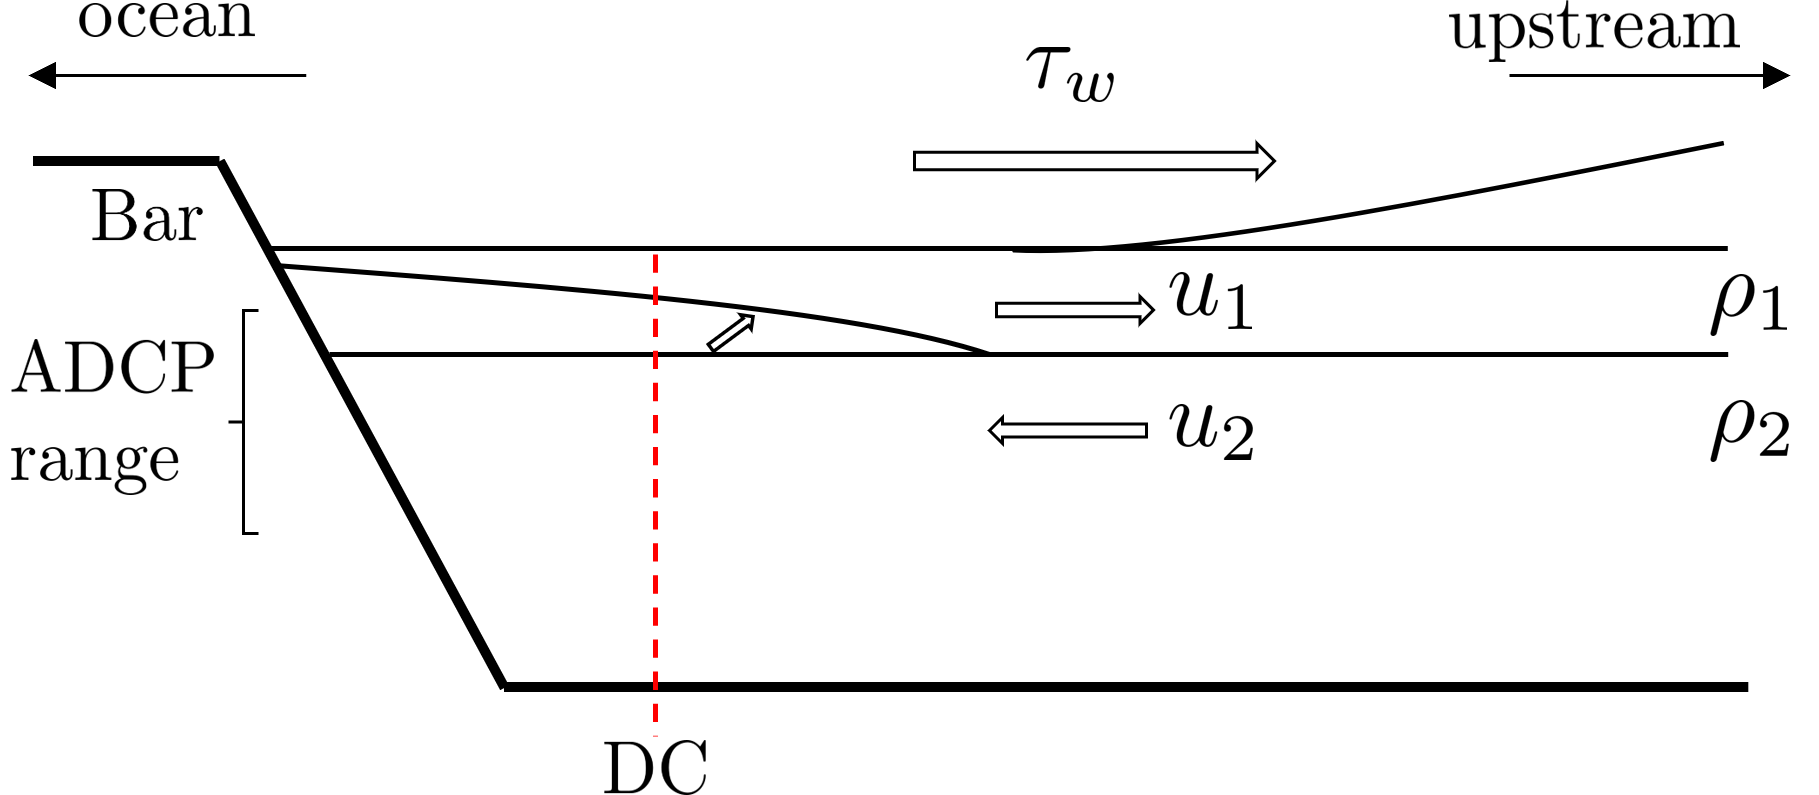
\includegraphics[width=0.6\textwidth]{Imagenes/ADCP_range.png}
    \caption{Scheme of the pycnocline tilt in an idealized estuary with the detected ADCP range in Pescadero.}
    \label{fig:adcp}
\end{figure}

Following the relaxation of the winds, the baroclinic pressure returns the estuary to its original state generating currents which are present mostly at the lower layers of the ADCP range (Fig. \ref{fig:velwind}). We observed negative velocities after the first relaxation between the two wind increases. First, negative velocities were present at the lower part, representing the return of the middle layer to its equilibrium position, while at the top velocities were positive, maybe showing the surface layer dynamics. After less than two hours there was a flip on the dynamics, at the upper part positive and the lower negative, meaning probably a seiche in the estuary.\\

\newpage
\begin{figure}[h!]
    \centering
    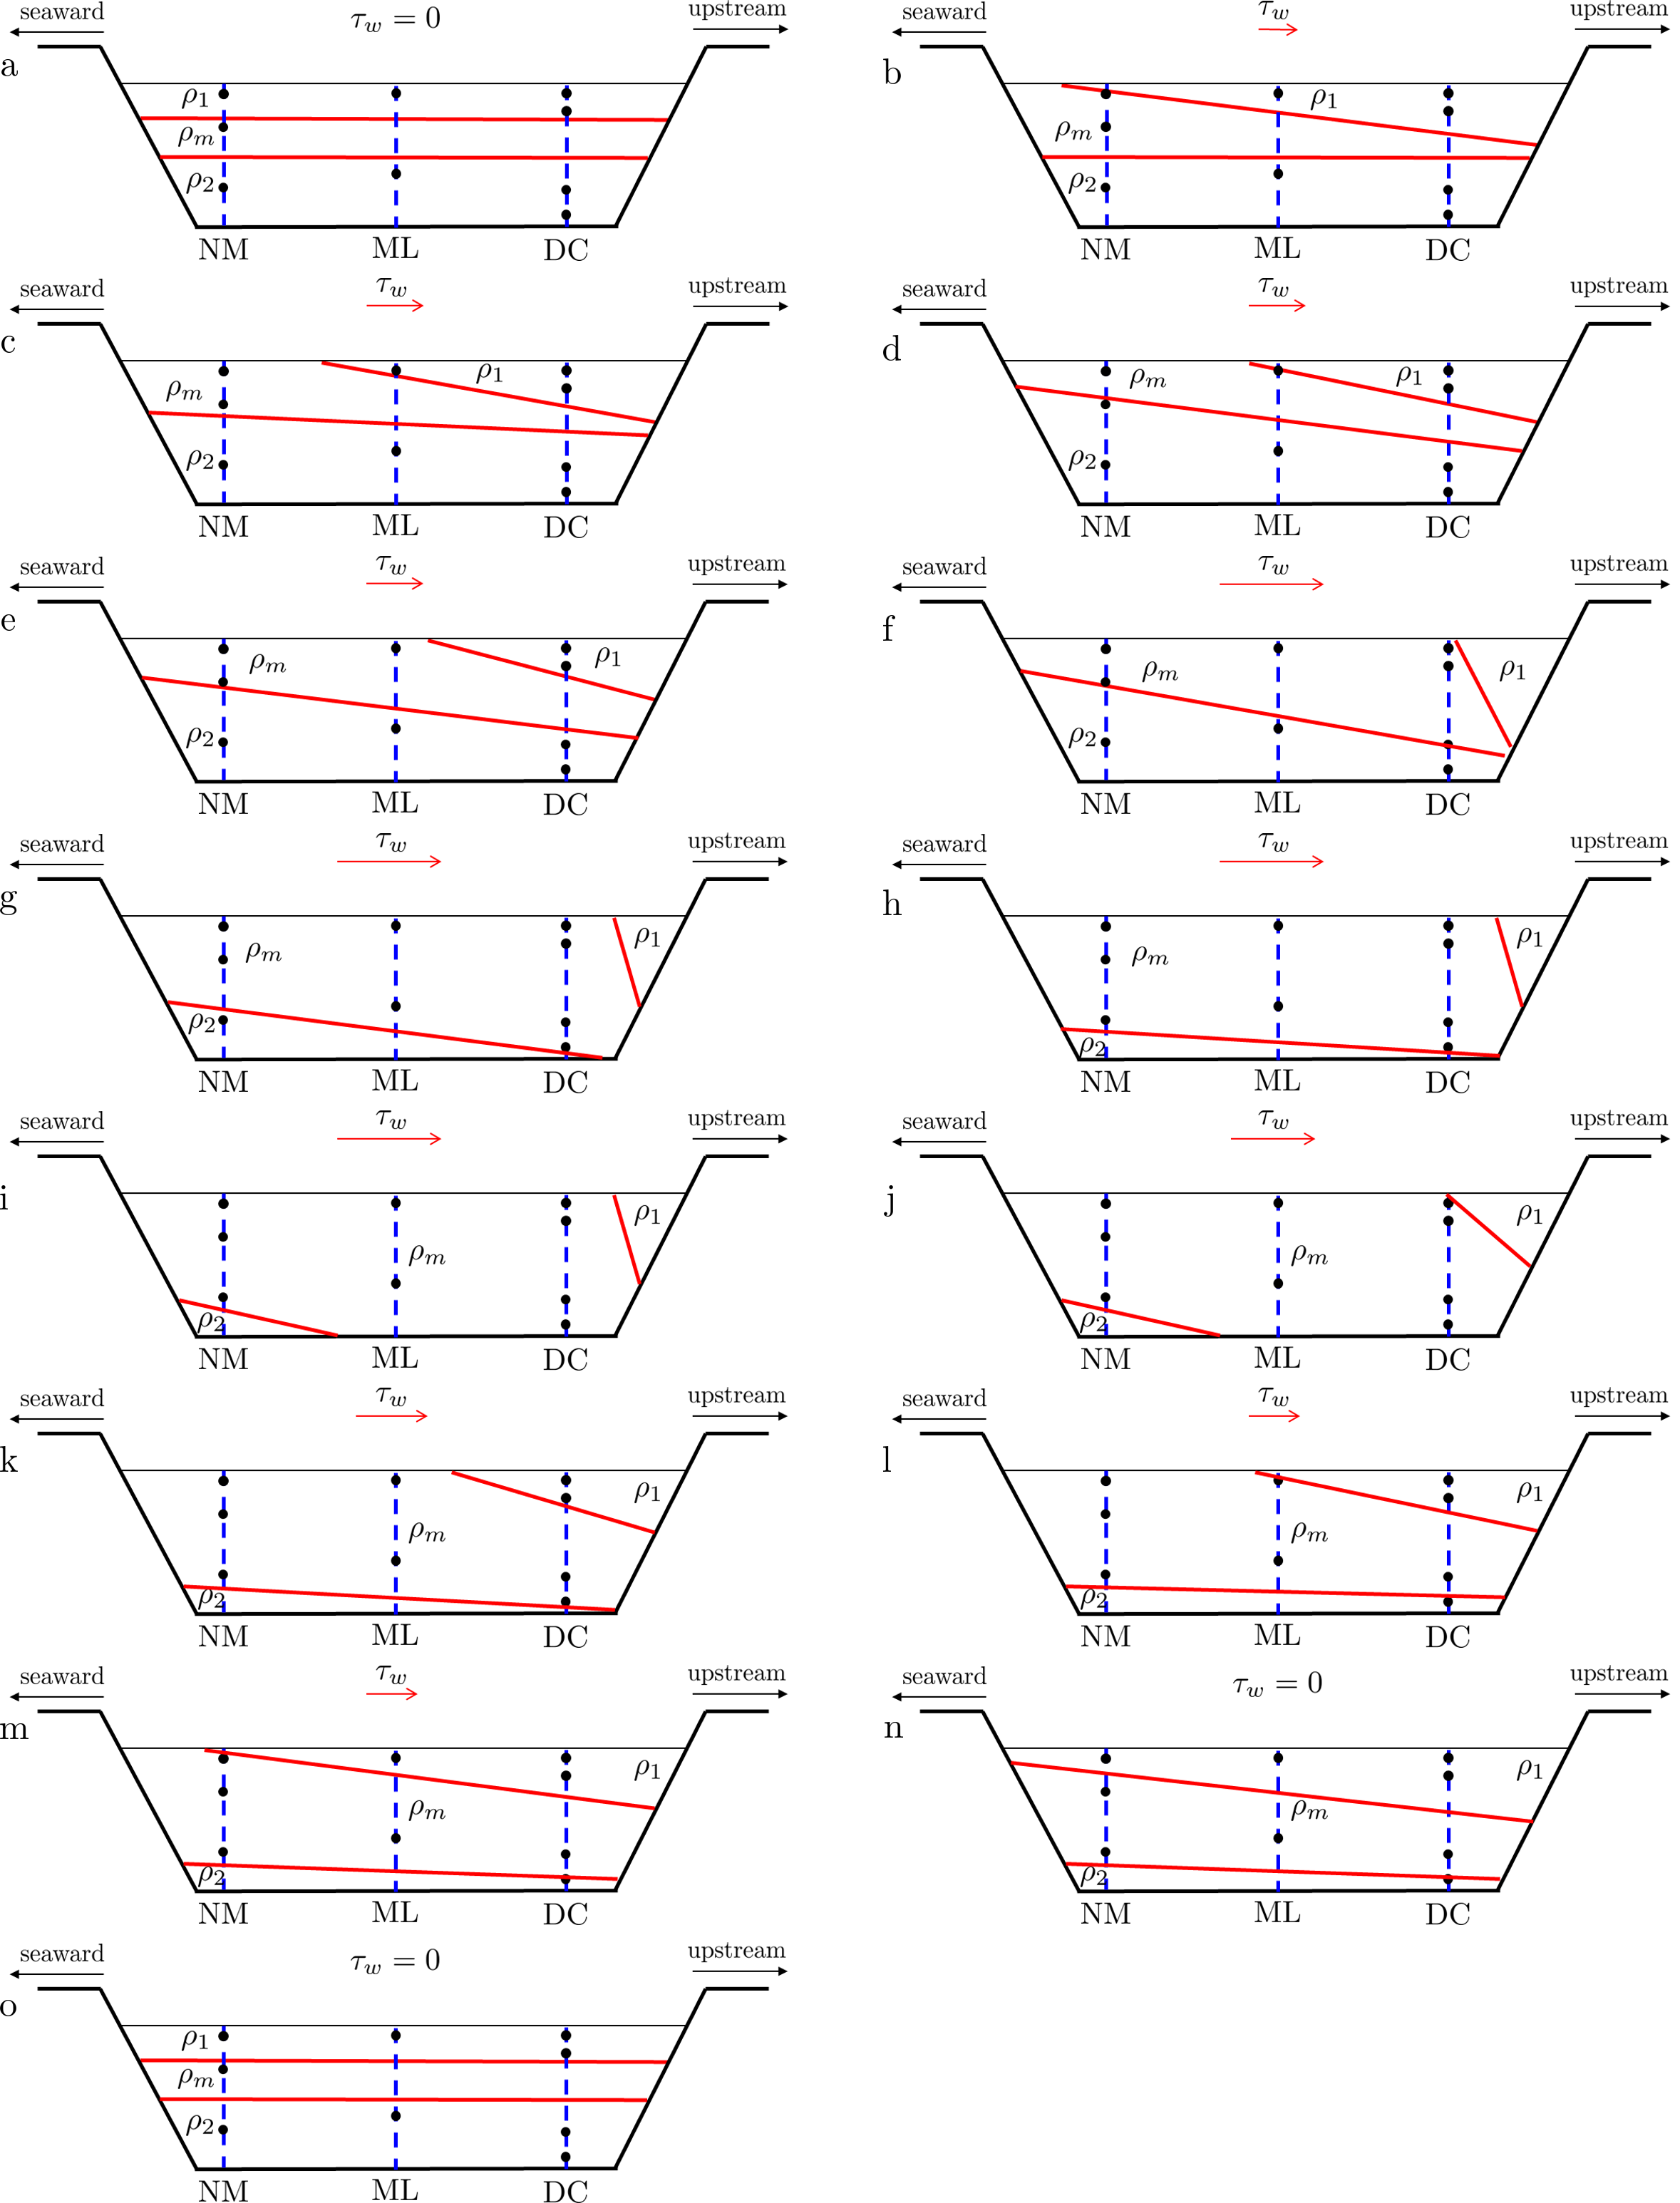
\includegraphics[width=0.95\textwidth]{Imagenes/wind_event.png}
    \caption{Movements of the density layers in Pescadero during the first wind event of the first period. The plots were constructed using the information given by the CTD.}
    \label{fig:wevent}
\end{figure}

\newpage
\begin{figure}[h!]
    \centering
    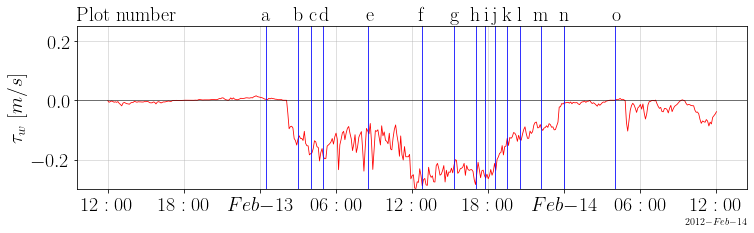
\includegraphics[width=0.95\textwidth]{Imagenes/wind_event2.png}
    \caption{Wind event that was plotted in Fig. \ref{fig:wevent} with the instants of each plot. }
    \label{fig:wevent2}
\end{figure}

After the second increase, we noticed a similar dynamic to after the first increase, but we didn't observe the flip happen. We observed that at the same time there was a wave overtopping event that probably affected the recirculation, but as it did not cause the same effect as before of negative velocities at the top its possible that it is not affecting the velocities with the same magnitude or it is overlapping the velocities of the relaxation changing its behavior. Another reason for the flip not happening is that the oscillation hadn't enough amplitude, so the seiche didn't happen.\\

Also, we studied the first wind event of the first period using the densities at locations NM, ML, and DC. In Fig. \ref{fig:wevent} we plotted the behavior of the layers according to the densities at different instants of time shown at Fig. \ref{fig:wevent2}. The sensors' positions were put in the horizontal center of the estuary and had a distance proportional to reality in the vertical for an easier estimation of the layers with the available information. During the wind event, the surface layer is moving landward due to the wind stress going in that direction, not being shown by any sensor at the biggest wind stress. The middle layer was occupying the water column for all the sensors during the peak of the wind event. The lower layer had an uncertain movement, but we drew it as the sensors were showing it, going in the same direction as the middle layer, not having the behavior of a third layer.\\

\subsection{Freshwater input}

The density time-series were showing a density decrease in time, especially at the bottom layer in NM and ML (Fig. \ref{fig:dens}), in DC we also observed a decrease but not in the deepest layer, in which we observed a light increase of density in the first period. The density decrease in time indicates a constant freshwater input. The parameter $\Delta \rho / \Delta z$ is also slowly changing in time, a fact that is not observable in Fig. \ref{fig:diff}, but what is clear is the change between before and after a wind event that is decreasing over time, showing that wind stress is affecting each time less the estuarine structure. The last statement is also noticeable in the Wedderburn number (Fig. \ref{fig:wedd}) where we observe in the last wind events W barely gets close to the threshold.\\

The destratification of the estuary could be a result of the freshwater constant input that is changing the density structure continuously in time. Also, it could be a result of the mixing that triggers the discharge increase during storm events, due to water's faster entrance to the estuary, which can induce interfacial instability \citep{Katopodes2018}. The discharge increase is only reflected in the estuary at the surface (Fig. \ref{fig:surf}) and is not very clear in the density, especially as it happens at the same time as a wind event in the first period and a wave overtopping event in the second period. It is possible that the rapid increase in the incoming flow generate mixing, although there is not enough evidence to say that this is happening.\\

Like we said before, the two registered freshwater inflow increases happened with other events at the same time, the first one during a wind event and the other while there was wave overtopping. That is why we cannot attribute the changes observed in $\hat{H}$, $dh/dt$ or $\Delta \hat{H}/\Delta x$ exclusively to discharge increase (Fig. \ref{fig:surf}). In Fig. \ref{fig:qh} we observe discharge versus the water level and the level change over time. The first one had a strong correlation until $Q$ started decreasing while $H_{DC}$ still increase. The second plot also has some correlation, but we observe $dh/dt$ is not increasing constant, so $Q$ did not affect constantly the same at the water level increase rate, but still, there is a strong relationship between them.\\

\begin{figure}[h!]
    \centering
    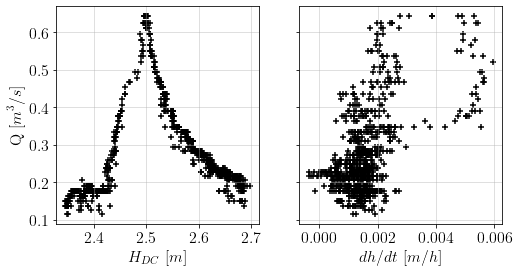
\includegraphics[width=0.8\textwidth]{Imagenes/qh.png}
    \caption{Discharge versus estuary height and discharge versus the height change in a 10-hour-frame for the period between 11 Feb. and 20 Feb..}
    \label{fig:qh}
\end{figure}

Fig. \ref{fig:mix_q} is showing the second discharge increase that happened at the same time as a wave overtopping event. We observed surface fluctuations in $\hat{H}$ while it was increasing and $\phi$ was increasing also, showing that Pescadero is stratifying instead of destratifying as was thought. When $Q$ reached its highest value, it began to decrease and then became constant, while $\phi$ kept increasing until the wind event when momentarily reached lower values. When the wind stopped $\phi$ did not reach the same value that before showing the wind event reduced stratification.\\

\begin{figure}[h!]
    \centering
    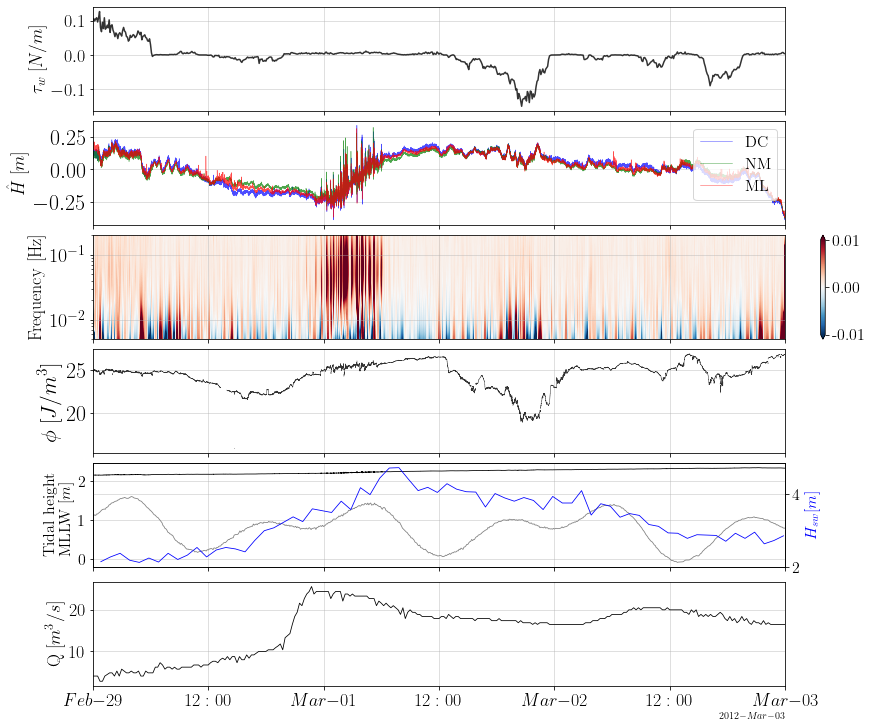
\includegraphics[width=\textwidth]{Imagenes/mix_q2.png}
    \caption{Time-series of wind stress ($\tau_w$), standardized depth ($\hat{H}$) in DC, NM, and ML locations, depth wavelet frequency analysis at DC, the potential energy anomaly ($\phi$), significant wave height in Halfmoon Bay (blue), and tidal height in San Francisco (gray), and freshwater discharge ($Q$). }
    \label{fig:mix_q}
\end{figure}

The freshwater inflow is affecting stratification in the medium term and not in short term, not causing mixing when it increases, different from wind stress. Discharge is affecting the estuary by constantly and slowly reducing density.\\

\subsection{Wave overtopping}

Wave overtopping is an event that happens during high tide and relatively high significant wave height, but also can depend on the wave period or the wave direction. To determine the factors involved in this process Fig. \ref{fig:WO} illustrates the tide level with significant wave height, dominant wave period, and dominant wave period direction as the estuary level rises. We noticed that two events happened with a significant wave height between 4 and 6 m and the others between 2 and 4 m. For the dominant wave period, we didn't observe a clear pattern, but the direction of the dominant period showed the events occurred between 300$^o$ and 325$^o$. \\

\begin{figure}[h!]
    \centering
    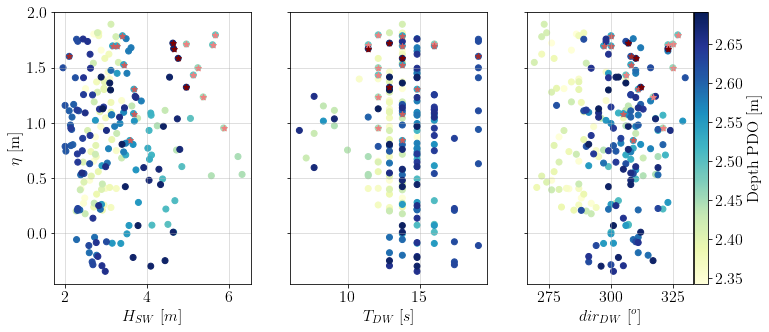
\includegraphics[width=\textwidth]{Imagenes/WO.png}
    \caption{Tide level ($\eta$) versus significant wave height ($H_{SW}$), dominant wave period ($T_{DW}$), and dominant wave period direction ($dir_{DW}$) with the water level of Pescadero (Depth PDO) in colors, during the period between 11 Feb. and 20 Feb.. Four wave overtopping events were selected as the most prominent of the period and were marked in the plot with reddish stars. }
    \label{fig:WO}
\end{figure}

As we already mentioned wave overtopping causes changes in surface velocities, which led us to believe that there would be mixing in the estuary during these events due to the turbulent entry of the waves over the sand bar. However, we couldn't find any evidence of it causing destratification or decrease of the $\phi$ in Fig. \ref{fig:mix_q}, probably because it wasn't an event big enough for the water level. \\

On the other hand, we observed a slow increase in density at the bottom layer of DC, which does not follow the same pattern of density decrease that the other locations had. In Fig. \ref{fig:mix_wo} there is a close-up of DC bottom density during the first period. First, we noticed that on 14 February there is an important wave overtopping event during which there is a negative spike in $\rho_{DC}$. After that, density started increasing but did not recover its value from before the spike. This could mean there was mixing due to the action of the waves, but as at the same time, there was a $Q$ increase we cannot attribute any driver in specific. It could be the action of both causing the spike.\\

\begin{figure}[h!]
    \centering
    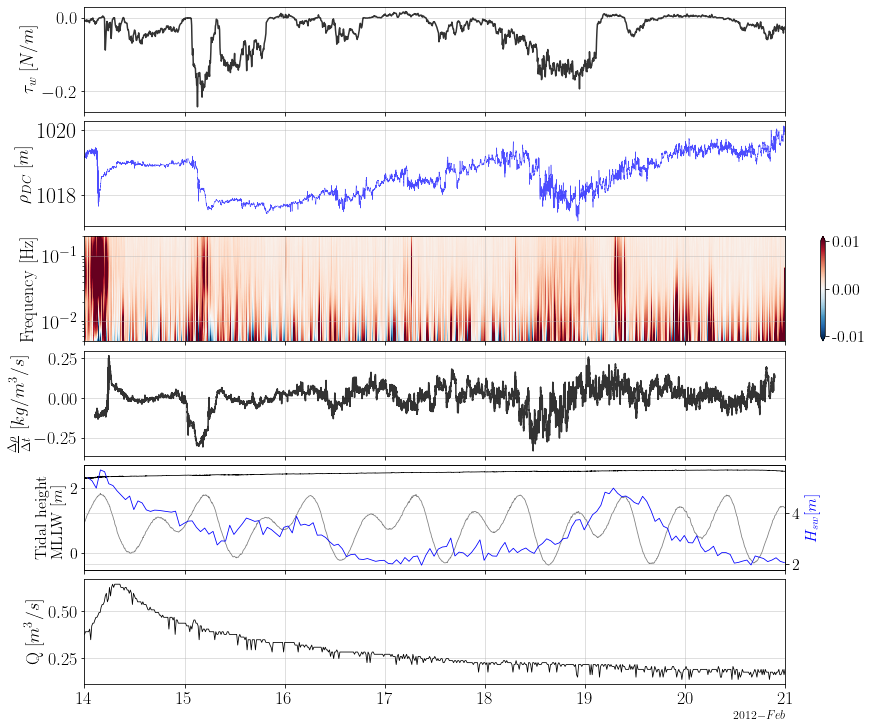
\includegraphics[width=\textwidth]{Imagenes/mix_wo.png}
    \caption{Time-series of wind stress ($\tau_w$), bottom density in DC location ($\rho_{DC}$), depth wavelet frequency analysis at DC, the change of density in a 10-hour time frame ($\Delta \rho / \Delta t$), significant wave height in Halfmoon Bay (blue), tidal height in San Francisco (gray), and Pescadero estuary water level (black) in MLLW datum, and freshwater discharge ($Q$). }
    \label{fig:mix_wo}
\end{figure}

After that, the wind would further reduce the density and, later, it would progressively increase. During that increase, we observed a smaller decrease during a wind event and another during a wave overtopping event on 17 February (Fig. \ref{fig:mix_wo}). By observing this we can say that there is mixing due to the turbulent inflow of waves into the estuary that affects the deeper layer.\\ 

Also, the saline water inflow from the wave overtopping events could be causing the increase in density at the bottom of DC. The baroclinic effect could be making the saltwater set at the bottom slowly after the waves, but also it is possible that there is not enough saline water to change salinity and a baroclinic effect alone is acting in Pescadero.\\


\end{document}